\documentclass{beamer}
%[aspectratio=169]   \usepackage[czech]{babel}
\usepackage{apo-lecture}
\usepackage{pdfpages}
\usepackage{pdfcomment}
\usepackage{listings}
\usepackage{array,multirow}

\subtitle{Lekce 05. Zřetězené zpracování\\Pipelining}
\author{Pavel Píša \phantom{xxxxxxx} Petr Štěpán \\ \small\texttt{pisa@fel.cvut.cz}\phantom{xxxx}\small\texttt{stepan@fel.cvut.cz}}
\begin{document}

\maketitle

\section{Zřetězené zpracování}

\begin{frame}
\frametitle{Todo}
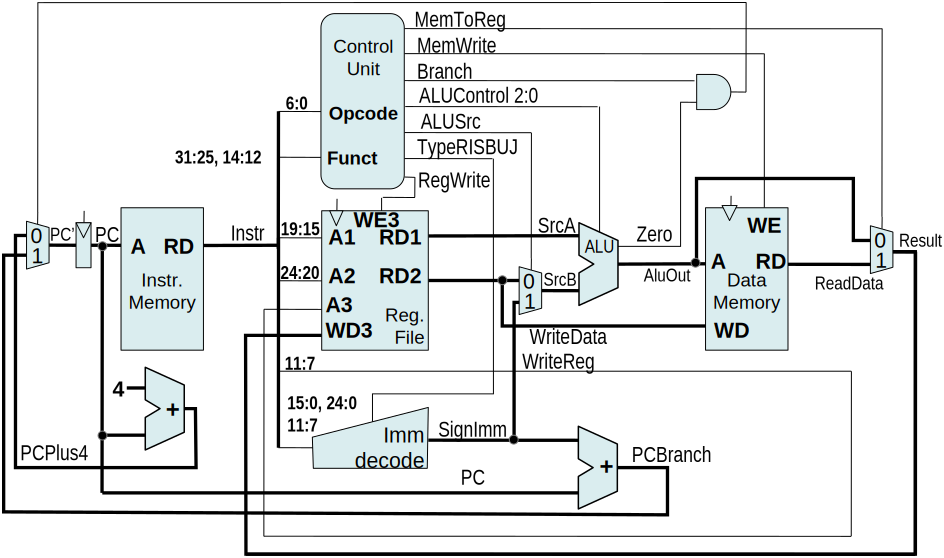
\includegraphics[width=0.95\textwidth]{single_cpu.pdf}
\end{frame}

\begin{frame}
\frametitle{Todo}
\includegraphics[width=0.95\textwidth]{cpu_clock.pdf}
\end{frame}

\begin{frame}
\frametitle{Todo}
\includegraphics[width=0.95\textwidth]{cpu_nopipe.pdf}
\end{frame}

\begin{frame}
\frametitle{Todo}
\includegraphics[width=0.95\textwidth]{cpu_pipe.pdf}
\end{frame}

\begin{frame}
\frametitle{Todo}
\includegraphics[width=0.95\textwidth]{cpu_ctrl_pipe.pdf}
\end{frame}

\begin{frame}
\frametitle{Todo}
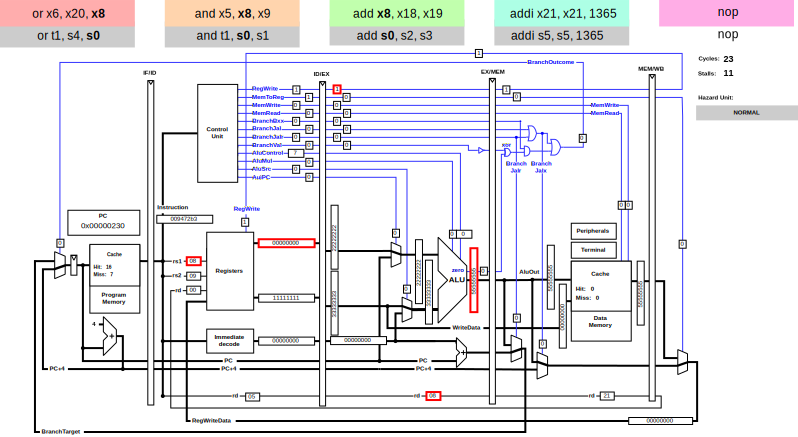
\includegraphics[width=0.95\textwidth]{hazard_qtrvsim.pdf}
\end{frame}

\begin{frame}
\frametitle{Todo}
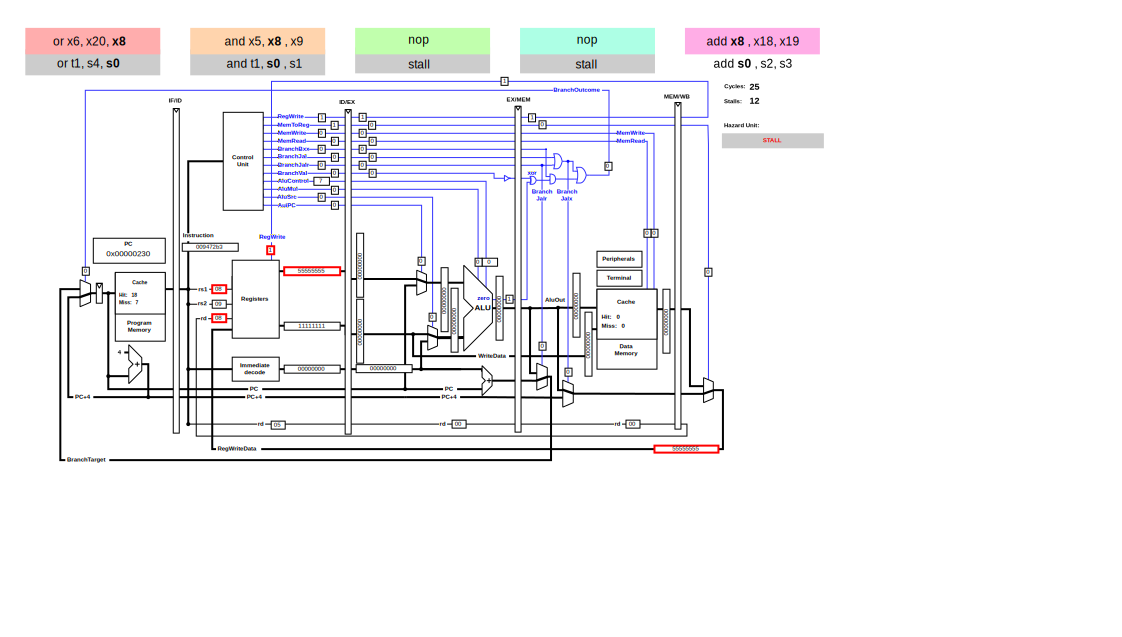
\includegraphics[width=0.95\textwidth]{hazard_stall_qtrvsim.pdf}
\end{frame}


\begin{frame}
\frametitle{Todo}
\includegraphics[width=0.95\textwidth]{forward_data.pdf}
\end{frame}

\begin{frame}
\frametitle{Todo}
\includegraphics[width=0.95\textwidth]{noforward_data.pdf}
\end{frame}

\begin{frame}
\frametitle{Todo}
\includegraphics[width=0.95\textwidth]{forward_hazard.pdf}
\end{frame}

\begin{frame}
\frametitle{Todo}
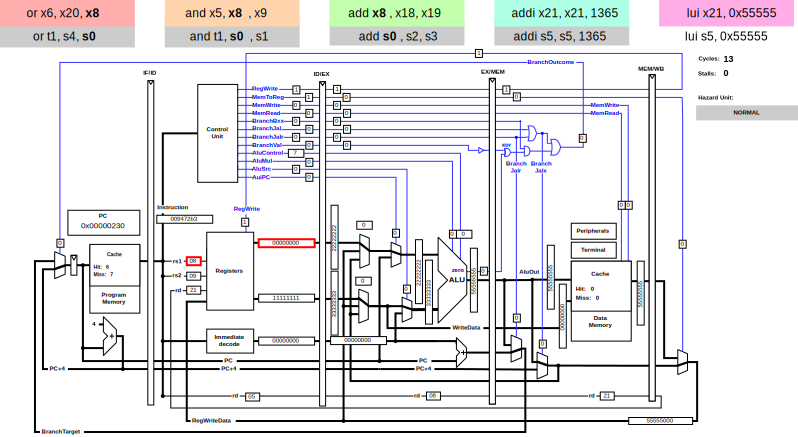
\includegraphics[width=0.95\textwidth]{hazard_forwarding.pdf}
\end{frame}

\begin{frame}
\frametitle{Todo}
\includegraphics[width=0.95\textwidth]{hazard_forwarding2.pdf}
\end{frame}

\begin{frame}
\frametitle{Todo}
\includegraphics[width=0.95\textwidth]{pipeline_stall.pdf}
\end{frame}

\begin{frame}
\frametitle{Todo}
\includegraphics[width=0.95\textwidth]{pipeline_stall2.pdf}
\end{frame}

\begin{frame}
\frametitle{Todo}
\includegraphics[width=0.95\textwidth]{cpu_fwd_stall.pdf}
\end{frame}

\begin{frame}
\frametitle{Todo}
\includegraphics[width=0.95\textwidth]{fig/hazard-stall-qtrvsim2.png}
\end{frame}

\begin{frame}
\frametitle{Todo}
\includegraphics[width=0.95\textwidth]{fig/hazard-stall-qtrvsim3.png}
\end{frame}

\begin{frame}
\frametitle{Todo}
\includegraphics[width=0.95\textwidth]{fig/hazard-stall-qtrvsim4.png}
\end{frame}

\begin{frame}
\frametitle{Todo}
\includegraphics[width=0.95\textwidth]{hazard_ctrl.pdf}
\end{frame}

\begin{frame}
\frametitle{Todo}
\includegraphics[width=0.95\textwidth]{hazard_ctrl2.pdf}
\end{frame}

\begin{frame}
\frametitle{Todo}
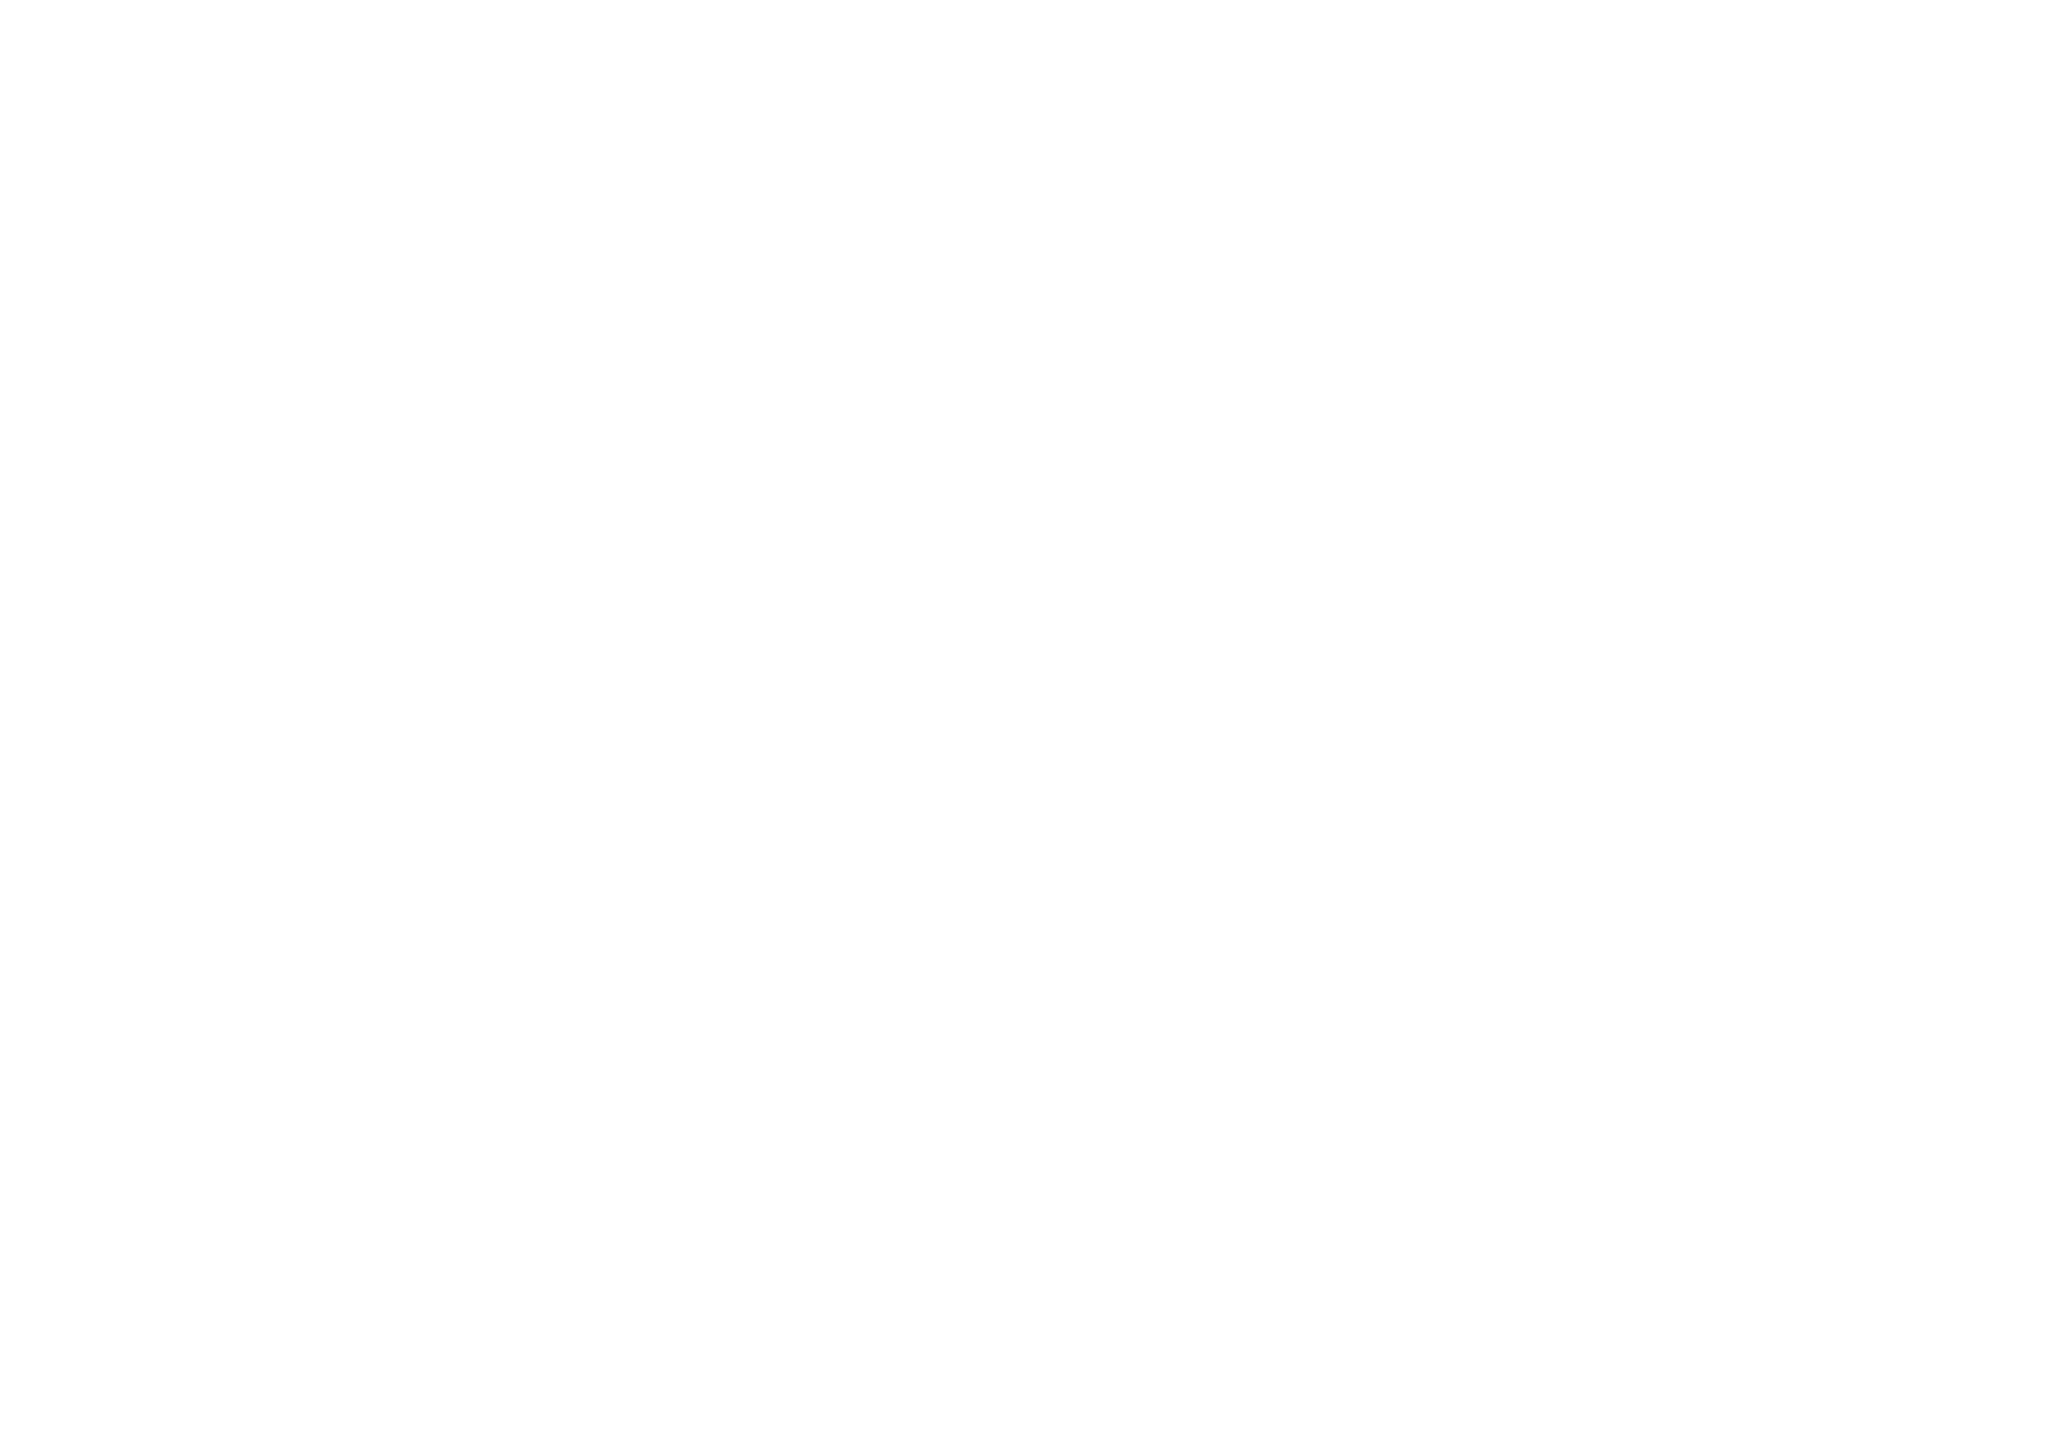
\includegraphics[width=0.95\textwidth]{cpu_branch_pred.pdf}
\end{frame}

\begin{frame}
\frametitle{Todo}
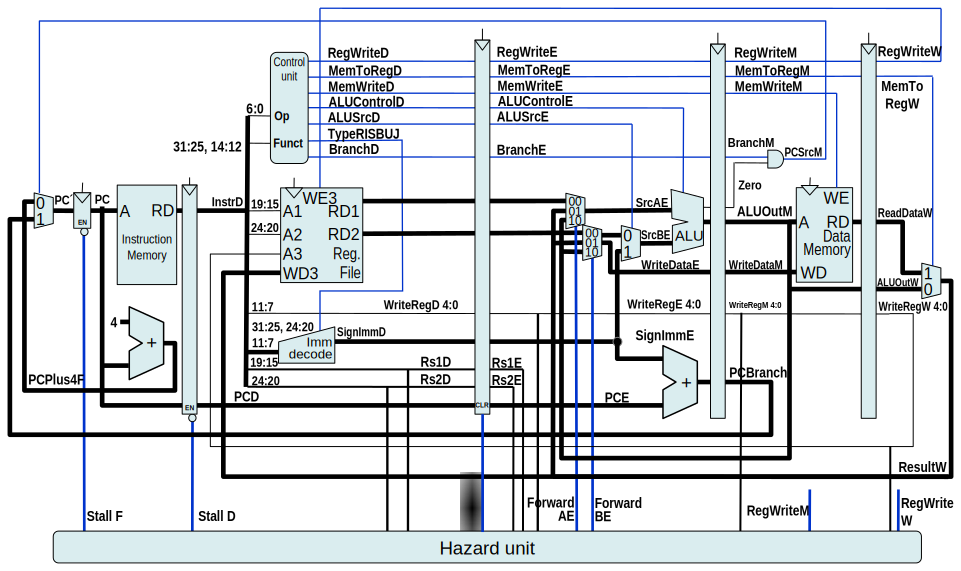
\includegraphics[width=0.95\textwidth]{cpu_final_design.pdf}
\end{frame}

\begin{frame}
\frametitle{Todo}
\includegraphics[width=0.95\textwidth]{cpu_design.pdf}
\end{frame}

\begin{frame}
\frametitle{Todo}
\includegraphics[width=0.95\textwidth]{cpu_design2.pdf}
\end{frame}

\begin{frame}
\frametitle{Todo}
\includegraphics[width=0.95\textwidth]{cpu_design3.pdf}
\end{frame}

\begin{frame}
\frametitle{Todo}
\includegraphics[width=0.45\textwidth]{fig/timing_clk.png}

\includegraphics[width=0.45\textwidth]{fig/timing_clk3.png}
\hfill 
\includegraphics[width=0.45\textwidth]{fig/timing_clk2.png}

\end{frame}





\end{document}

